% Block Diagram for TTL IC Multiplexer 74HC153
% Author: Ramón Jaramillo.
\documentclass[tikz,border=10pt,12pt,x11names]{standalone}
%%%<
\usepackage{verbatim}
%%%>
\usetikzlibrary{calc,arrows}
\usepackage{tikz}
\usepackage[]{circuitikz} % TiKZ Library for US Logic Circuits.
\usetikzlibrary{circuits.logic.US} % TiKZ Library for US Logic Circuits.

\usepackage{tikz}
\usetikzlibrary{circuits.logic.US} % TiKZ Library for US Logic Circuits.
\begin{document}
	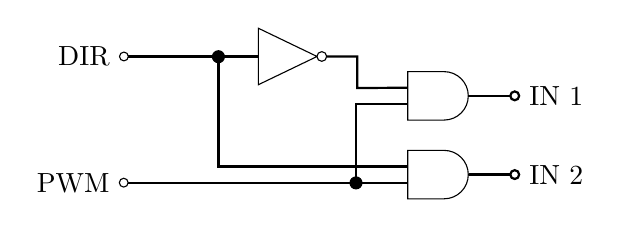
\begin{tikzpicture}[every path/.style={},>=triangle 45,circuit logic US, every circuit symbol/.style={}]
	% Logic Gates
	\node[and gate,inputs={nn}, point right] (and1) at (2,-1)    {};
	\node[and gate,inputs={nn}, point right] (and2) at (2,-2)    {};
	\node[not gate, point right] (not1) at (0,-0.5) {};
	
	
	\draw (not1.output)[thick] -| (1,-0.9) -- (and1.input 1);
	
	%Outputs
	\draw (and1.output) [thick] -- (3,-1) node[ocirc,label={right:IN 1} ](in1) {};
	\draw (and2.output) [thick]-- (3,-2) node[ocirc,label={right:IN 2} ](in2) {};
	
	
	%inputs DIR
	\draw ([xshift=-1.7cm]not1.input) [thick] -| ([xshift=-0.5cm]not1.input) -- (not1.input) {};
	\draw ([xshift=-0.5cm]not1.input)[thick] |- (and2.input 1) {};
	
	% input PWM
	\draw ([xshift=-3.6cm]and2.input 2) [thick] -- (and2.input 2){};
	\draw ([xshift=-0.65cm]and2.input 2) [thick] |- (and1.input 2){};
	
	\draw ([xshift=-1.7cm]not1.input) node[ocirc,label={left:DIR} ](dir) {};
	\draw ([xshift=-3.6cm]and2.input 2) node[ocirc,label={left:PWM} ](pwm) {};
	
	% dots
	\draw [*-]([xshift=-0.5cm,yshift=0.08cm]not1.input){};
	\draw [*-]([xshift=-0.65cm,yshift=0.08cm]and2.input 2){};
	\end{tikzpicture}
\end{document}